\section{Instruction Level Parallelism}\label{capitolo3}
Come abbiamo visto nei capitoli precedenti in una macchina fornita di pipeline possiamo dimostrare come il numero di clock necessari per eseguire un'istruzione sia:
$$\begin{array}{rcl}
CPI_{pipeline} & = & CPI_{ideale}+ Stalli \ Strutturali + Stalli \ Data \ Hazard + \\
&& Stalli \ di \ Controllo + Stalli \ di \ Memoria
\end{array}$$
La riduzione di uno qualsiasi dei termini sulla destra da in modo che $CPI_{pipeline}$ si avvicini sempre più al $CPI_{ideale}$. Il caso migliore si ha quando il throughput è massimo ed è uguale a 1
$$IPC_{ideale} = 1; \\ CPI_{ideale} = 1$$
Tuttavia si hanno dei limiti alle performance dovuti ai diversi tipi di \emph{rischi (Hazards)}, questi possono essere di diversa natura:
\begin{itemize}
\item \textbf{Strutturali:} si possono risolvere tramite l'introduzione di nuovo hardware.
\item \textbf{Dati:} necessitano di \emph{forwarding} e di una schedulazione del codice a livello di compilazione.
\item \textbf{Controllo:} Early evaluation, Branch Delay Slot, Predizione dei salti statica e dinamica.
\end{itemize}
Inoltre per le pipeline più profonde (superpipelining) questi problemi sono accentuati.\\
In questo capitolo ci concentreremo su come incrementare il \emph{CPI} oltre il valore ideale; per fare ciò però dobbiamo prima capire quali sono gli \emph{hazard} sui dati che possiamo incontrare.
\subsection{Tipi di Hazards sui dati}
Gli hazard innanzitutto sono quei conflitti che avvengono a tempo di esecuzioni e sono generati da dipendenze a livello di istruzione. Consideriamo l'esecuzione di un istruzione generale di questo tipo:
$$r_k \leftarrow (r_i) \ op \ (r_j)$$
Possiamo avere tre tipi di dipendenza a livello di istruzione come mostrato in \figurename\,\ref{fig:datadep}
\begin{figure}[htb]
\centering
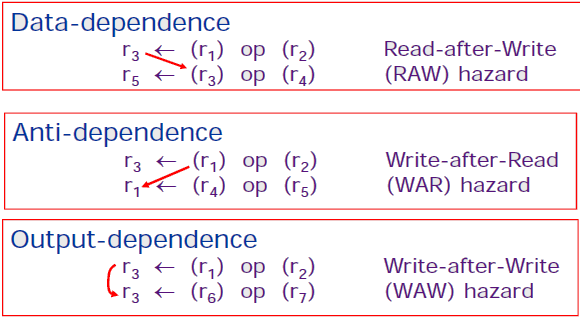
\includegraphics[scale=0.4]{img/datadep.png}
\caption{Esempi di dipendenza dei dati}\label{fig:datadep}
\end{figure}
\subsection{Parallelismo a livello di istruzione}
Per raggiungere livelli di performance maggiori è necessario estrarre dai programmi maggiore parallelismo, questo si traduce in pipeline con più uscite (\emph{multiple-issue}). Per fare ciò è necessario individuare e risolvere le dipendenze, inoltre è utile riordinare (\emph{schedule}) le istruzioni in modo da ottenere un maggiore parallelismo a tempo di esecuzione compatibilmente con le risorse a disposizione.\\
Per dare una definizione formale del parallelismo a livello di istruzione (\emph{ILP}) possiamo dire che 
\begin{center}
\textit{ILP = Sfruttare la potenziale esecuzione sovrapposta di istruzione non correlate}
\end{center}
Tale sovrapposizione è possibile tutte le volte che:
\begin{itemize}
\item Non abbiamo degli \emph{Hazard} di tipo strutturale
\item Non abbiamo \emph{Hazard} di tipo RAW, WAR oppure WAW
\item Non abbiamo \emph{Hazard} di controllo
\end{itemize}
Un esempio di sistema \emph{dual-issue} è mostrato in \figurename\,\ref{fig:dualpipe} e \figurename\,\ref{fig:dualmips}
\begin{figure}
\centering
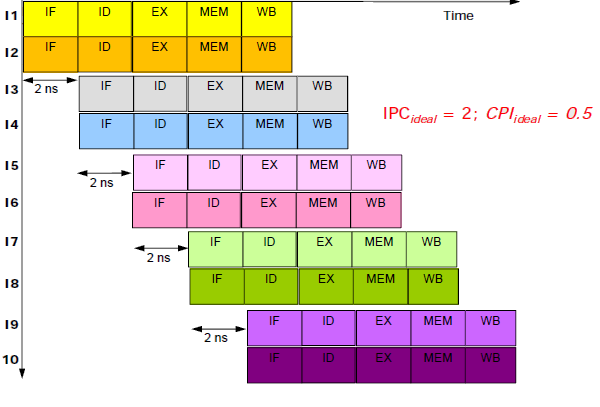
\includegraphics[scale=0.5]{img/dualpipe.png}
\caption{Esecuzione di istruzione in una pipeline dual-issue}\label{fig:dualpipe}
\end{figure}
\begin{figure}
\centering
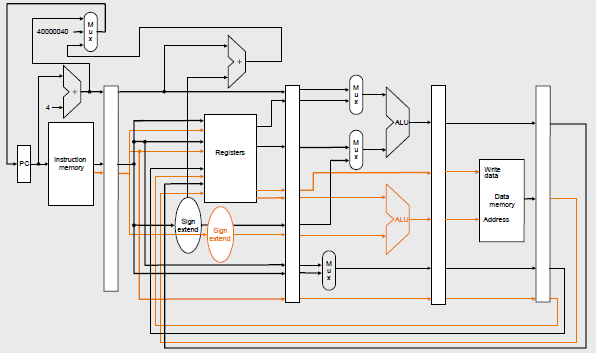
\includegraphics[scale=0.5]{img/dualmips.png}
\caption{Schema hardware per una pipeline dual-issue con una unità ALU/BR e una unità load/store}\label{fig:dualmips}
\end{figure}
In pipeline di tipo multiple-issue il $CPI_{ideale}$ risulta essere $<1$ ad esempio considerando il caso ottimale di un processore \emph{2-issue} abbiamo che ad ogni ciclo di clock vengono completate 2 istruzioni questo significa che:
$$IPC_{ideale} = 2; \\ CPI_{ideale} = 0.5$$
Uno degli aspetti più critici nel caso di ILP è la determinazione delle dipendenze tra le istruzioni; infatti, se due istruzioni sono dipendenti tra loro esse non possono essere eseguite in parallelo ma dovranno essere eseguite in sequenza o al più in parziale sovrapposizione. Possiamo distinguere tre tipi di dipendenza:
\begin{itemize}
\item Dipendenza dei dati (Vera dipendenza)
\item Dipendenza dei nomi
\item Dipendenza di controllo
\end{itemize}
\paragraph{Dipendenza dei nomi}
Tale dipendenza avviene quando due istruzioni usano lo stesso registro o la stessa area di memoria (chiamata \emph{nome}) ma non esiste alcun flusso di dati tra queste due istruzioni. Possiamo individuare due tipi di dipendenza dai nomi tra due istruzioni \textbf{i} e \textbf{j} nelle quali \textbf{i} precede \textbf{j}
\begin{itemize}
\item \textbf{Antidipendenza:} quando l'istruzione \emph{j} scrive un registro che l'istruzione \textbf{i} legge; l'ordine originale delle istruzioni deve essere preservato per essere sicuri che \textbf{i} legga il valore corretto (WAR).
\item \textbf{Output dipendenza:} quando \textbf{i} e \textbf{j} scrivono lo stesso registro o la stessa area di memoria; l'ordine delle istruzioni deve essere rispettato per essere sicuri che il valore finale sia quello scritto da \textbf{j}
\end{itemize}
In realtà la dipendenza dai nomi non è una vera e propria dipendenza in quanto non vi è alcuno scambio di valori tra le istruzioni; se il \emph{nome} usato nell'istruzione può essere cambiato non ci sono conflitti. Tuttavia per quanto riguarda le aree di memoria è molto più difficile localizzare questo tipo di conflitto infatti due indirizzi possono essere diversi ma puntare alla stessa area (\emph{memory disambiguation}) mentre una rinominazione dei registri risulta molto più semplice.
La rinominazione può essere effettuata sia staticamente dal compilatore sia in modo dinamico dall'hardware.
\paragraph{Dipendenze dei dati}
Le dipendenze dei dati possono potenzialmente generare dei \emph{Data Hazard} ma l'impatto che questi hazard hanno in termini di stalli e tecniche di eliminazione degli stalli sono caratteristiche specifiche della pipeline e non dipendono dalla dipendenza.
Le \emph{RAW} sono le uniche vere dipendenze sui dati che abbiamo.
Le dipendenze sono una caratteristica del programma mentre gli \emph{hazard} sono specifiche della pipeline.
\paragraph{Dipendenze di controllo}
Le dipendenze di controllo sono determinate dall'ordinamento delle istruzioni e sono preservate da due proprietà:
\begin{itemize}
\item Le istruzioni devono essere eseguite nell'ordine del programma per assicurare che un'istruzione che si trova prima di un salto venga eseguita prima del salto.
\item Individuazione degli \emph{hazard di controllo} per assicurare che un'istruzione che dipende da un salto non sia eseguita prima di conoscere la direzione del salto.
\end{itemize}
Sebbene preservare il controllo delle dipendenze sia un modo semplice per preservare l'ordine del programma esso non è così essenziale da dover essere preservato.
\subsubsection{ILP in pratica}
Dalla trattazione appena fatta possiamo ricavare due proprietà importanti per verificare la correttezza di un programma (e che in realtà preservano sia le dipendenze dei dati che quelle di controllo):
\begin{itemize}
\item \textbf{Data flow:} il flusso dei valori dei dati attraverso le istruzioni deve produrre il risultato corretto.
\item \textbf{Exception behavior:} preservare il comportamento delle eccezioni che significa che qualsiasi cambiamento nell'ordine di esecuzione delle istruzioni non deve cambiare come le eccezioni sono sollevate dal programma.
\end{itemize}
Esistono due tecniche fondamentali per supportare e implementare l'\emph{ILP}, lo \textbf{scheduling dinamico} che dipende dall'hardware per localizzare il parallelismo e lo \textbf{scheduling statico} che fa affidamento sul software per individuare possibili parallelismi. La prima soluzione è quella più utilizzata in ambito desktop e server.\\
Consideriamo ora un processore di tipo \emph{single-issue} lo stage IF precede quello EXE e le istruzioni possono essere prelevate sia dall'\emph{Instruction Register} sia da una coda di istruzioni pendenti. La fase di esecuzione può richiedere più cicli di clock in base al tipo di operazione.\\
\paragraph{Scheduling dinamico}
Il problema principale è quello che non si può nascondere una dipendenza dai dati senza causare uno stallo nell'esecuzione della pipeline. Una soluzione è quella di permettere alle istruzioni situate dopo lo stallo di procedere; l'hardware deve riordinare dinamicamente l'esecuzione delle istruzioni per dar in modo di ridurre gli stalli. Per fare ciò è necessario permettere un esecuzione fuori ordine e una fase di commit finale.\\
L'hardware riordina l'esecuzione delle istruzioni per ridurre il numero degli stalli della pipeline mentre mantiene il \emph{data flow} e \emph{exception behavior}. I vantaggi principali di questa tecnica sono il fatto di permettere una gestione di alcuni casi in cui esistono delle dipendenze non note al tempo della compilazione, inoltre permette di semplificare la complessità del compilatore ed infine permette di compilare il codice affinché esso venga eseguito efficientemente anche su pipeline diverse. Questi vantaggi tuttavia hanno un costo che comporta un significativo incremento della complessità dell'hardware, un incremento dei consumi e può generare delle eccezioni imprecisate.
Tale soluzione è utilizzata soprattutto nei \emph{Processori Super-scalari}
\paragraph{Scheduling statico}
In questo caso il compilatore utilizza dei sofisticati algoritmi per individuare e organizzare il codice in modo da sfruttare l'\emph{ILP}, per fare ciò analizza i \textbf{basic block} e ricerca il parallelismo in questi seppur esso sia minimo (15\% - 25\%), ed inoltre sfrutta il parallelismo tra diversi \emph{basic block}. Un limite a questa tecnica è però la dipendenza dai dati presente nei vari blocchi base. Tipicamente questa tecnica è sfruttata dai processori \textbf{VLIW} (\emph{Very Long Instruction Word}) i quali si aspettano del codice privo di dipendenze dal compilatore.\\
Il limite principale di questa tecnica è dato dall'impredicibilità dei salti, dalla latenza della memoria, dalla dimensione del codice e dalla complessità del compilatore.
\subsubsection{Esecuzione super-scalare e VLIW}
Passando al caso \emph{multi-issue} la questione si complica anche se le prestazioni migliorano come vediamo in \figurename\,\ref{fig:superscalar}, infatti si vogliono eseguire più istruzioni per ogni ciclo di clock; per fare ciò è necessario prelevare più istruzioni per ciclo dall'IR e questo dipende dalla banda a disposizione. La cosa più difficile però risulta essere l'analisi delle dipendenze dei dati e di controllo per le istruzioni da eseguire.
\begin{figure}[htb]
\centering
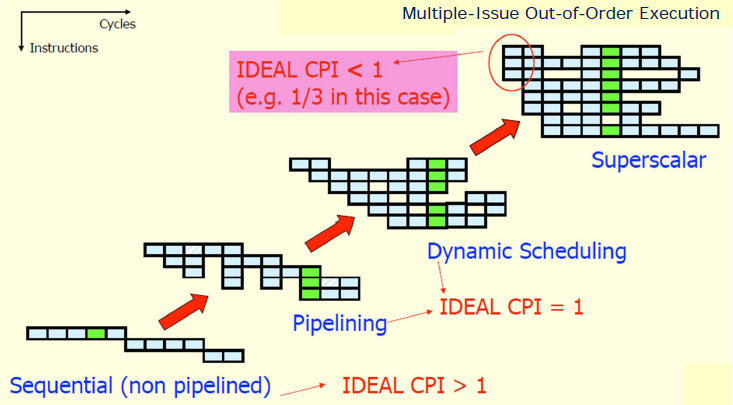
\includegraphics[scale=0.5]{img/superscalar.png}
\caption{Confronto di prestazioni tra architetture}\label{fig:superscalar}
\end{figure}
In \figurename\,\ref{fig:superstrut} vediamo come è strutturato un processore super-scalare nel quale possiamo notare le diverse unità per l'esecuzione di istruzioni parallele come le due ALU o l'unità per le istruzioni di load/store, e l'unità per il riordino delle istruzioni.\\
\begin{figure}[htb]
\centering
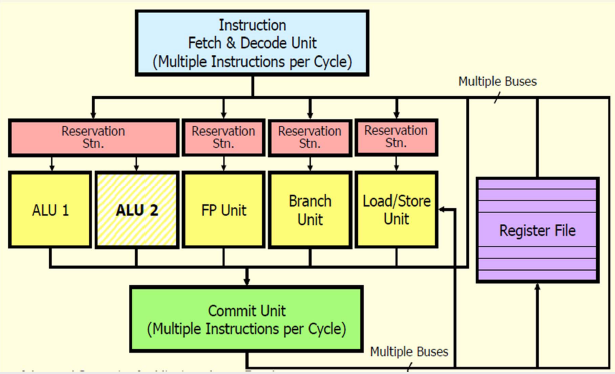
\includegraphics[scale=0.5]{img/superstrut.png}
\caption{Struttura di un prcessore superscalare}\label{fig:superstrut}
\end{figure}
Per decidere quali istruzioni mandare in esecuzione si utilizza lo \emph{Scheduler dinamico} il quale per ogni ciclo di clock analizza quali sono le dipendenze e per fare ciò la sua complessità è molto alta, nell'ordine del quadrato delle possibili istruzioni come mostrato in \figurename\,\ref{fig:dinamicscheduler}.
\begin{figure}[htb]
\centering
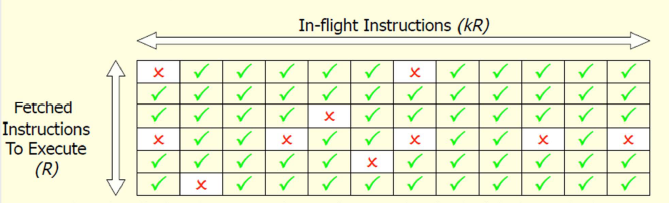
\includegraphics[scale=0.5]{img/dinamicscheduler.png}
\caption{Tabella delle dipendenze in uno scheduler dinamico}\label{fig:dinamicscheduler}
\end{figure}
Esiste un limite al numero di istruzioni che possono essere analizzate durante un singolo ciclo di clock, infatti i limiti principali dei processori super-scalari riguardano tutti lo scheduler dinamico in quanto esso è molto costoso in termini di area in quanto la sua logica è molto complessa, il tempo di clock dipende dal tempo di analisi delle istruzioni ed infine la verifica del design dello scheduler è molto complessa.
Queste limitazioni portano a delle limitazioni in termini di istruzioni che possono essere eseguite simultaneamente. Attualmente in realtà esistono dei processori a 6-issue anche se molto rari, più normalmente sono di tipo 4-issue o minori in quanto è troppo difficile trovare 8 o addirittura 16 istruzioni indipendenti in un singolo ciclo.\\
La famiglia di processori multi-issue che sfruttano lo scheduler statico sono, invece, i processori VLIW (\emph{Very Long Instruction Word}) nei quali è il compilatore che decide cosa far fare ad ogni istruzione per ogni ciclo di clock come si vede in \figurename\,\ref{fig:vliw}.
\begin{figure}[htb]
\centering
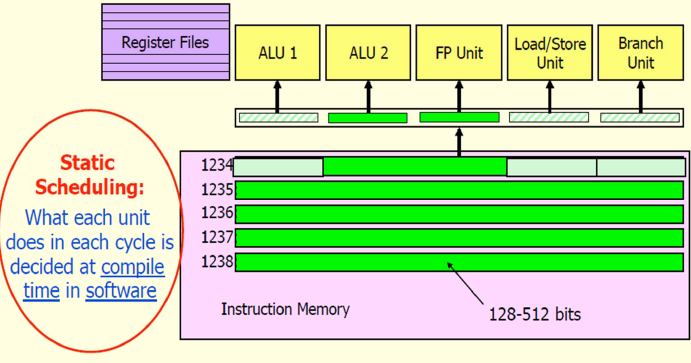
\includegraphics[scale=0.5]{img/vliw.png}
\caption{Scheduler statico nel caso di processori VLIW}\label{fig:vliw}
\end{figure}
I processori di tipo super-scalare sono utilizzati soprattutto in ambito desktop e server, mentre i processori VLIW sono utilizzati soprattutto in ambito embedded in quanto la decisione sull'esecuzione è presa a compile-time e non è necessario aggiungere dell'area per lo scheduler dinamico.
\subsection{Scoreboard}
Come abbiamo visto fino ad ora lo scheduling dinamico è il meccanismo più utilizzato nei sistemi general purpose per sfruttare il parallelismo tra le istruzioni. Tale meccanismo però ha diverse tecniche di implementazione, una di queste è lo \textbf{Scoreboard}. Lo \emph{Scoreboard} divide il normale stage ID in due stage per permettere l'esecuzione delle istruzioni nell'ordine più efficiente. Questi due stage sono:
\begin{itemize}
\item Lo stage \emph{issue} che si occupa di decodificare le istruzioni e di verificare eventuali hazard strutturali.
\item Lo stage \emph{read operands} (RR) che si occupa di risolvere i data hazard ritardando eventualmente la lettura dei registri.
\end{itemize}
Grazie a questo meccanismo le istruzioni vengono eseguite quando non hanno alcuna dipendenza o non esistono degli hazard strutturali non verifica però una eventuale priorità delle istruzioni.\\
Per spiegare la struttura dello \emph{Scoreboard} dobbiamo innanzitutto definire quando un'istruzione si dice in \textbf{esecuzione}. Possiamo distinguere quando un'istruzione inizia la sua esecuzione e quando essa la termina durante questi due istanti l'istruzione si dice in \emph{esecuzione}. In una pipeline possono esistere molte istruzioni in esecuzione nello stesso momento, questo richiede che esistano più unità funzionali. Quello che noi analizzeremo è la struttura di un \textbf{CDC 6600} nel quale le istruzioni vengono immesse in ordine ma vengono eseguite e completate in un ordine casuale. L'architettura di questo sistema è mostrata in \figurename\,\ref{fig:scorearch}
\begin{figure}[htb]
\centering
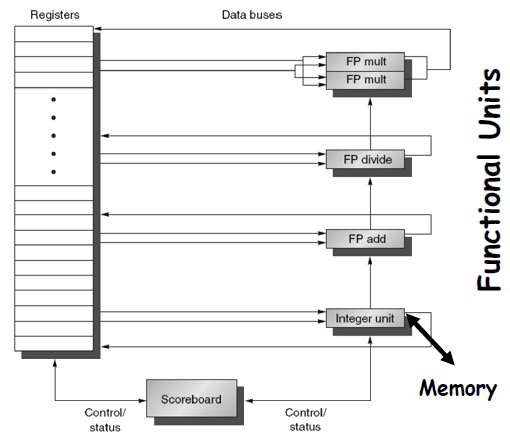
\includegraphics[scale=0.5]{img/scorearch.png}
\caption{Architettura di un sistema \emph{Scoreboard}}\label{fig:scorearch}
\end{figure}
Nella pipeline di uno scoreboard le fasi ID, EXE e WB sono sostituite da quattro stage. Lo stage ID è diviso in due parti, la prima chiamata \textbf{Issue} la quale decodifica l'istruzione e controlla eventuali hazard strutturali, la seconda chiamata \textbf{Read Operands} che attende fino alla risoluzione degli hazard sui dati. Lo scoreboard fa in modo che le istruzioni eseguite siano prive di dipendenze. Come abbiamo visto le istruzioni vengono prelevate in ordine dallo stage \emph{Issue} ma da quell'istante esse possono essere ordinate in qualsiasi modo, infatti durante lo stage \emph{read operands} esse possono essere bloccate o bypassate, inoltre, la latenza di esecuzione può variare tra le diverse unità funzionali.\\
Un completamento fuori ordine può portare però a hazard di tipo WAR o WAW che tuttavia possono essere facilmente risolti infatti per i WAR è sufficiente:
\begin{itemize}
\item Bloccare il \emph{write back} finché i registri non vengono letti
\item Effettuare la lettura dei registri soltanto durante la fase di \emph{Read Operands}
\end{itemize}
Mentre per risolvere i WAW è sufficiente individuare l'hazard e bloccare l'esecuzione delle istruzioni dipendenti successive fino a quando esse non vengono concluse.\\
L'individuazione e la risoluzione degli hazard è centralizzata nello \emph{scoreboard}; ogni istruzione attraversa lo scoreboard dove viene aggiornata una tabella delle dipendenze, a questo punto lo scoreboard determina quando l'istruzione può leggere i registri ed iniziare la sua esecuzione. Se un'istruzione non può cominciare immediatamente la sua esecuzione lo scoreboard monitora ogni cambiamento e decide quando l'istruzione può andare in esecuzione. Infine, lo scoreboard, controlla quando l'istruzione scrive il risultato dentro i registri di destinazione.\\
Un problema che si viene a creare quando si accetta il completamento delle istruzioni fuori ordine è quello della preservazione del comportamento delle eccezioni; una soluzione è quella di assicurarsi che nessuna istruzione possa generare una eccezione finché il processore non conosce esattamente l'istruzione che ha sollevato l'eccezione. Un'eccezione si dice \emph{imprecisa} se lo stato del processo nell'istante in cui viene sollevata una eccezione non è uguale a quello del caso in cui l'istruzione sia eseguita in ordine; un'eccezione imprecisa si può verificare quando la pipeline ha già completato delle istruzioni che sequenzialmente si trovano dopo l'istruzione che ha sollevato l'eccezione, oppure se non ha ancora completato istruzioni che sequenzialmente la precedono.
\paragraph{I quattro stadi dello Scoreboard}
Analizziamo ora in dettaglio i quattro stadi dello Scoreboard. Il primo stadio è quello di \emph{Issue} nel quale le istruzioni vengono decodificate e si verificano gli eventuali hazard strutturali e quelli di WAW. Le istruzioni lasciano questo stage in ordine, se l'unità funzionale necessaria per eseguire l'istruzione è libera e non esistono altre istruzioni che hanno lo stesso registro di destinazione (no WAW) lo stage issue inoltra l'istruzione all'unità funzionale e aggiorna la sua struttura interna. In caso contrario lo stage ferma l'istruzione fino a quando tutti gli hazard sono stati risolti. Ogni qualvolta lo stage di issue ferma un istruzione il buffer tra IF e Isuue si riempe. Nel caso il buffer sia singolo IF si blocca e attende l'Issue nel caso invece il buffer sia a coda l'IF si blocca solo nel caso in cui la coda sia piena.\\
Lo stage \emph{Read Operands} attende la risoluzione dei data hazard e legge i registri. Un registro risulta disponibile quando non ci sono istruzioni attive precedenti che scrivono su di esso oppure se un unità funzionale scrive il suo risultato in tale registro. Quando i registri sono disponibili lo scoreboard comunica all'unità funzionale di leggere i registri. Gli RAW hazard vengono risolti dinamicamente in questa fase.\\
Lo stage \emph{execution} è lo stage composto dalle unità funzionali; durante questo stage le unità funzionali svolgono le diverse operazioni, quando il risultato è pronto viene notificato allo scoreboard. Le unità funzionali sono caratterizzate da una latenza variabile, il tempo per iniziare l'esecuzione è variabile in quanto è il tempo necessario per leggere i diversi registri, i tempi per effettuare una load/store variano in base ai cache HIT/MISS.\\
L'ultimo stage è denominato \emph{Write Result}, in questa fase si controllano eventuali hazard di tipo WAR e si termina l'esecuzione scrivendo il risultato nel registro di destinazione.
\paragraph{Lo Scoreboard in pratica}
Lo scoreboard è formato da tre unità fondamentali:
\begin{itemize}
\item Instruction status
\item Functional Unit status: il quale indica lo stato delle unità fondamentali tramite diversi indici
\begin{description}
\item[Busy:] indica se la FU è occupata oppure no
\item[Op:] indica l'operazione da eseguire
\item[$F_i$:] registro di destinazione
\item[$F_j,F_k$:] registri sorgenti
\item[$Q_j,Q_k$:] indicano quale FU sta tenendo occupato il registro corrispondente
\item[$R_j,R_k$:] sono dei flag che indicano lo stato dei registri sorgenti.
\end{description}
\item Register Result status: indica quale FU dovrà scrivere sui registri di destinazione.
\end{itemize}
Per un esempio completo si rimanda alle slide dell'insegnante.
\subsection{Algoritmo di Tomasulo}
Un altro tipo di algoritmo da sfruttare per lo scheduling dinamico è l'algoritmo di \emph{Tomasulo} introdotto da IBM tre anni dopo il CDC 6600 lo scopo di tale algoritmo è sempre quello di ottenere prestazioni elevate senza l'utilizzo di speciali compilatori.\\
A differenza dello Scoreboard tuttavia il meccanismo di controllo e di buffer è distribuito sulle diverse unità funzionali. I buffer associati alle unità funzionali sono chiamate \emph{Reservation Station}. I registri nelle istruzioni sono sostituiti da valori o puntatori alle reservation station è possibile così il renaming dei registri. In questo modo si evitano anche eventuali hazard di tipi WAR e WAW; inoltre esistono più \emph{RS} che registri e questo permette delle ottimizzazioni che il compilatore non può fare. Infine il risultato delle FU non transita dai registri bensì viene diffuso a tutte le altre FU tramite un \emph{Common Data Bus}. Le operazioni di Load e Store sono trattate come normali FU . L'architettura necessaria per implementare l'algoritmo di Tomasulo è mostrata in \figurename\,\ref{fig:tomahw} mentre la struttura di una unità funzionale è mostrata in \figurename\,\ref{fig:fuhw}
\begin{figure}
\centering
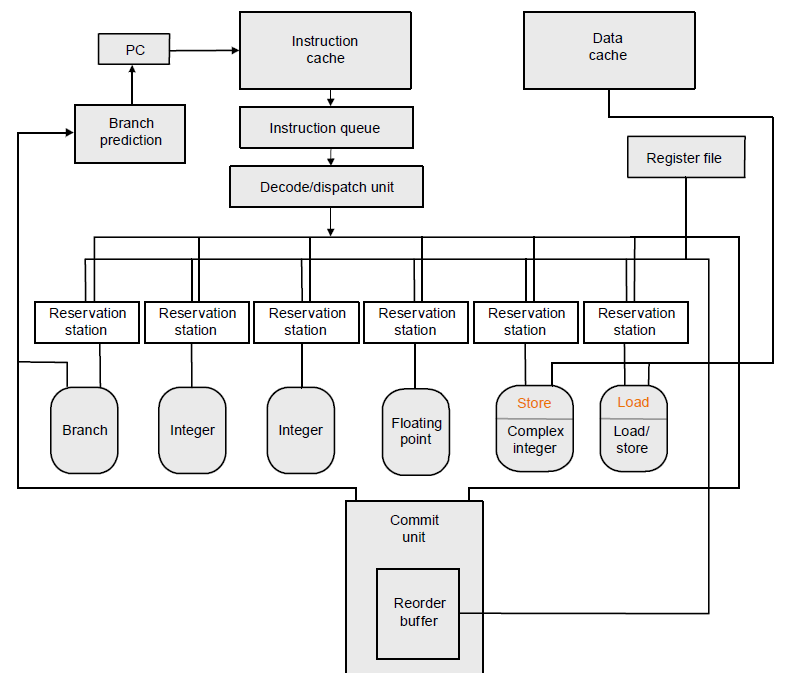
\includegraphics[scale=0.5]{img/tomahw.png}
\caption{Architettura per l'algoritmo di Tomasulo}\label{fig:tomahw}
\end{figure}
\begin{figure}
\centering
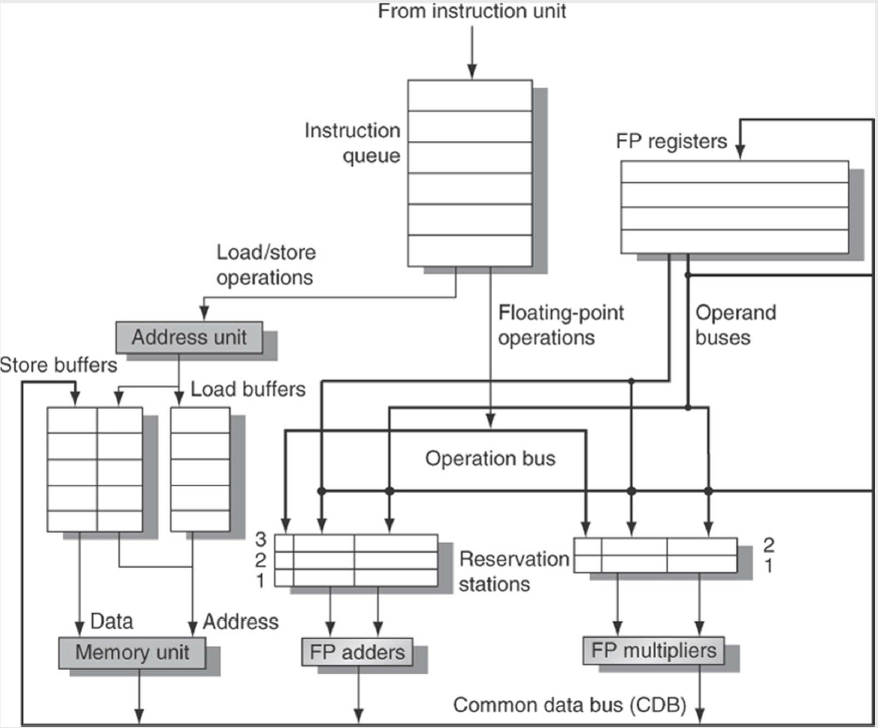
\includegraphics[scale=0.5]{img/fuhw.png}
\caption{Architettura di un'unità funzionale}\label{fig:fuhw}
\end{figure}
I vari campi che compongono una reservation station sono:
\begin{description}
\item[Tag:] identifica quale RS è coinvolta.
\item[Busy:] identifica se la RS è occupata.
\item[OP:] Identifica il tipo di operazione eseguita dal componete.
\item[$V_j,V_k$:] Valori contenuti nei registri; per la \emph{load}  $V_j$ contiene il valore dell'offset.
\item[$Q_j,Q_k$:] Puntatori alle RS che producono i valori $V_j,V_k$ se il valore è uguale a 0 l'operando è già disponibile. 
\end{description}
Si noti che solo uno dei due campi \emph{V} e \emph{Q} è disponibile per ogni operando in un determinato istante.\\
Il register file e lo Store buffer hanno un campo \emph{Value (V)} e uno \emph{Puntatore (Q)} il quale punta al numero della \emph{reservation station} che produce il risultato da immagazzinare, se questo puntatore è uguale a zero allora non ci sono istruzioni attive e il valore contenuto nel RF/Buffer è quello corretto.
Nel caso di Load buffer abbiamo un campo \emph{Address (A)} e un campo \emph{Busy}; il campo \emph{A} mantiene le informazioni riguardanti gli indirizzi calcolati nelle operazioni di Load/Store, all'inizio contiene le informazioni sull'offset poi, una volta calcolato, contiene l'indirizzo effettivo.
\subsubsection{Gli stadi dell'algoritmo di Tomasulo}
\paragraph{Il primo stadio: ISSUE}
Durante questo stadio si preleva un'istruzione \emph{I} dalla testa della coda delle istruzioni (\textbf{in-order issue}). Si controlla se la RS associata a quell'istruzione è vuota altrimenti si attende (controllo sugli structural hazard). Nel caso gli operandi non siano ancora disponibili si tiene traccia della FU che produce tali operandi (puntatore Q). Durante questa fase si effettua anche il \emph{Rename} dei registri in modo tale da evitare eventuali \emph{WAR}, infatti, se un istruzione \emph{I} scrive un registro \emph{$R_x$} e un istruzione $K$ già prelevata legge tale registro $K$ conosce già il valore di $R_x$ e lo ha immagazzinato nella sua RS oppure conosce quale operazione produce tale valore. Inoltre si evitano anche eventuali WAW in quanto le istruzioni sono prelevate in ordine.
\paragraph{Secondo stadio: Esecuzione}
Quando entrambi gli operandi sono disponibili si esegue l'operazione; nel caso in cui non siano pronti invece si controlla il \emph{Common Data Bus} in attesa del risultato; ritardando l'esecuzione si evitano eventuali RAW. Si noti come più istruzioni possono diventare eseguibili allo stesso istante per la stessa FU a questo punto bisogna verificare la disponibilità dell'unità funzionale. Le RAW hazard sono molto meno incisive in quanto sono gestite a livello di RS e non è necessario attendere il \emph{write back} sul register file.\\
Per quanto riguarda le istruzioni di load e di store l'esecuzione avviene in due passi, nel primo passo si calcola l'effettivo indirizzo di destinazione e si memorizza nel buffer, nel secondo passo in caso di load si esegue l'operazione non appena l'unità è disponibile nel caso della store si attende invece che il dato da immagazzinare sia disponibile.\\
Per preservare il comportamento dell'esecuzione nessuna istruzione può cominciare l'esecuzione fino a quando i branch precedenti non sono stati eseguiti. Se si usano tecniche di predizione la CPU deve conoscere se la predizione è corretta prima di procedere.
\paragraph{Terzo stadio: Write result}
Quando un risultato è disponibile esso viene scritto sul \emph{Common Data Bus} e da qui copiato sia sul RF sia su tutte le RS che attendono questo risultato. Il \emph{Common Data Bus} è un bus di tipo data+source composto da 64 bit di dati e 4 bit per la sorgente in questo modo le FU possono effettuare un lookup associativo.
\subsubsection{Alcuni dettagli}
Le operazioni di load e di store attraversano un'unità funzionale per il calcolo dell'indirizzo effettivo prima di procedere con le vere e proprie operazioni di load e di store. La load necessita di una seconda fase per accedere alla memoria mentre invia il risultato al RF e alle RS durante lo stage \emph{Write Result}. La store, invece completa la sua esecuzione durante lo stage \emph{Write Result} nel quale scrive i dati sul buffer.
Le operazioni di load e di store possono essere eseguite in  ordine differente purché esse accedano a differenti aree di memoria, in caso contrario possono presentarsi problemi di WAR (scambio tra load e store), di RAW (scambio tra store e load) oppure di WAW (scambio tra due store) invece le load possono essere scambiate liberamente. Per identificare questo tipo di anomalie il calcolo degli indirizzi di tutte le operazioni deve essere calcolato dalla CPU e quindi secondo l'ordine del programma.\\
Prendiamo il caso di una load eseguita fuori ordine con una store precedente ed assumiamo che il calcolo dell'indirizzo sia eseguito con l'ordine del programma. Quando l'indirizzo della load è calcolato esso viene comparato con i campi \emph{A} dello \emph{Store Buffer} nel caso vi sia un match la load non viene inviata allo Load Buffer fino a quando il conflitto non è risolto. Le operazioni di store invece verificano la presenza di conflitti sia nello Store Buffer che nel Load Buffer.
\subsubsection{Tomasulo in pratica}
Per un esempio completo si rimanda alle slide dell'insegnante per il funzionamento dell'algoritmo.
\subsubsection{Tomasulo vs Scoreboard}
Al contrario dello scoreboard l'algoritmo di Tomasulo ha una finestra di prelevamento delle istruzioni minore (5 vs 12) in entrambi i casi non si hanno hazard di tipo strutturale nel prelevamento delle istruzioni, nel caso di Tomasulo questi sono bloccati a livello di RS mentre nel caso dello Scoreboard a livello di FU. Tomasulo è più efficiente per quanto riguarda la risoluzione di WAW e di WAR che vengono risolti tramite renaming mentre per lo Scoreboard sono necessari alcuni stalli; inoltre, in Tomasulo il risultato di una FU è distribuito a tutte le altre tramite il Common Data Bus mentre nello scoreboard è necessario attendere che il risultato sia scritto nei registri di destinazione. Il controllo in Tomasulo è distribuito ed è possibile effettuare un loop unrolling al contrario dello Scoreboard. Tuttavia i limiti di Tomasulo risiedono nella sua complessità e alla limitazione delle prestazioni del COmmon Data Bus; inoltre il parallelismo è ridotto a causa dei salti.
\subsection{Register Renaming}
\subsubsection{Renaming implicito}
Analizziamo ora un piccolo codice di esempio che rappresenta un ciclo
\begin{verbatim}
Loop:  	LD		F0	0	R1
		MULTD	F4	F0	F2
		SD		F4	0	R1
		SUBI	R1	R1	#8
		BNEZ	R1	Loop
\end{verbatim}
ed assumiamo che la moltiplicazione abbia una latenza di 4 cicli, che la prima volta che viene effettuata la load si abbia un overhead di 8 cicli (cache miss) mentre nelle successive la latenza sia di 1 ciclo (cache hit), infine, assumiamo che la branch prediction predica che il salto sia effettuato.\\
Come abbiamo visto nel paragrafo precedente l'algoritmo di Tomasulo fornisce il \emph{register renaming} in modo implicito tramite le \emph{reservation station} le quali "bufferizzano" gli operandi delle istruzioni per evitare eventuali problemi di WAW e di WAR. Questo permette a iterazioni diverse di utilizzare registri fisici diversi (\textbf{dynamic loop unrolling}), inoltre, permette di sostituire i registri statici con dei puntatori dinamici che fanno in modo di incrementare praticamente la dimensione del register file. Questo permette alle istruzioni di procedere e, tramite l'uso della branch prediction di prelevare più istruzioni di iterazioni diverse.\\
Per un esempio di questo meccanismo si rimanda alle slide della professoressa riportiamo di seguito solo il passaggio dell'algoritmo al ciclo di clock 14 (\figurename\,\ref{fig:ciclo14})nella quale si nota come sia stato possibile effettuare un loop unrolling e come tale loop venga gestito in modo implicito infatti le operazioni del primo loop hanno tutte come registro base $R1 = 80$ mentre il secondo loop abbia come registro base $R1 = 72$.\\
\begin{figure}
\centering
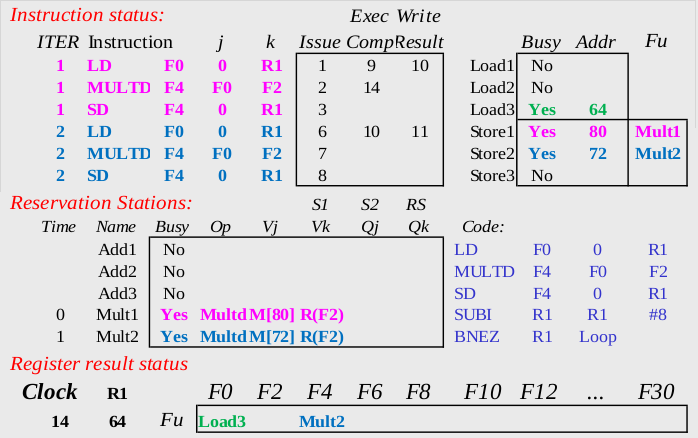
\includegraphics[scale=0.5]{img/ciclo14.png}
\caption{Algoritmo di Tomasulo all'istante 14}\label{fig:ciclo14}
\end{figure}
Il problema di questa tecnica è che necessita di prelevare le istruzioni \emph{in ordine} in quanto un prelevamento fuori ordine ci può portare ad avere WAR e RAW che in realtà non esistono. Tuttavia il meccanismo funziona bene nel caso di prelevamento di un unica istruzione. La situazione cambia completamente nel caso di prelevamento di istruzioni multiple in un singolo ciclo di clock, infatti, è necessario disporre di porte multiple  per la \emph{rename table} e dobbiamo essere in grado di effettuare il rename su diverse istruzioni contemporaneamente. Dobbiamo inoltre fornire istruzioni a più \emph{reservation station} nello stesso ciclo di clock e questo comporta l'utilizzo di 2x porte in lettura e 1x porte in scrittura. Il prelevamento delle istruzioni in sequenza è il vero collo di bottiglia nel caso di istruzioni multiple per singolo ciclo di clock.\\
Il completamento fuori ordine riduce notevolmente la nostra possibilità di avere delle eccezioni \emph{precise} in quanto il register file può contenere risultati di istruzioni successive e magari non contenere risultati di istruzioni precedenti e non ancora completate.
In questo contesto sarebbe necessario effettuare un \emph{rollback} del register file in modo da avere un'eccezione \emph{precisa} ovvero nella quale tutte le istruzioni precedenti a quella che ha generato l'eccezione hanno "committato" il loro risultato e nessuna istruzione successiva ha "committato" il risultato
\subsubsection{Renaming esplicito}
Come abbiamo appena visto tomasulo fornisce il renaming in modo implicito tramite l'utilizzo delle reservation station. Quello che vogliamo fare ora è capire come implementare un renaming dei registri in modo esplicito. Per fare questo innanzitutto dobbiamo tener conto che dobbiamo utilizzare un maggior numero di registri fisici rispetto a quelli specificati dall'ISA. Il principio chiave è quello di allocare una nuova destinazione fisica per ogni istruzione che scrive un risultato. Questa tecnica è molto simile alla trasformazione effettuata dal compilatore chiamata \emph{Static Single Assignment (SSA)} ma in questo caso viene effettuata dallo hardware. Con questa tecnica si rimuovono tutte le possibilità di avere WAR o WAW. In \figurename\,\ref{fig:rftoprf} vediamo come il \emph{Register File Fisico} sia molto più grande di quello standard, inoltre, notiamo la presenza di una tabella denominata \emph{Freelist} nella quale sono memorizzati i registri fisici che non sono utilizzati e che sono quindi \emph{liberi}. 
\begin{figure}[htb]
\centering
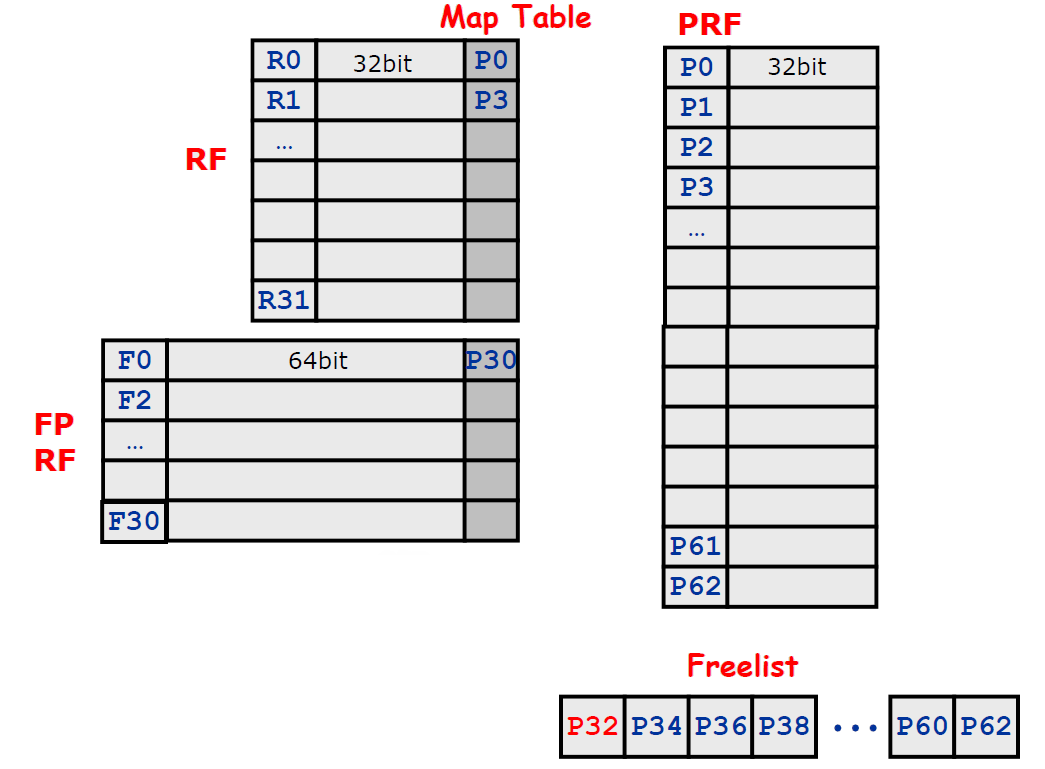
\includegraphics[scale=0.5]{img/rftoprf.png}
\caption{Associazione tra RF e RF fisico}\label{fig:rftoprf}
\end{figure}
Per implementare questo meccanismo è sufficiente tenere traccia dell'associazione dei registri tramite una \emph{tabella di traduzione} come mostrato in \figurename\,\ref{fig:translation}.
\begin{figure}[htb]
\centering
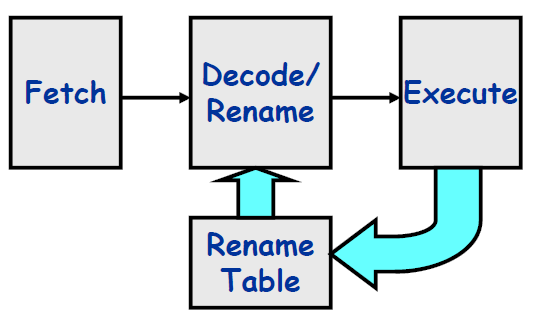
\includegraphics[scale=0.5]{img/translation.png}
\caption{Meccanismo di register renaming}\label{fig:translation}
\end{figure}
Quando un'istruzione deve scrivere un risultato in un registro esso viene sostituito da un nuovo registro preso dalla \emph{freelist}. Un registro torna a far parte della \emph{freelist} quando non è più usato da nessuna istruzione.\\
I vantaggi di questa tecnica sono il disaccoppiamento del concetto di renaming da quello di scheduling, la pipeline è esattamente uguale a quella dello MIPS, con la possibilità di implementare scheduling dinamici (Tomasulo o Scoreboard) la possibilità di prelevare più istruzioni per singolo ciclo di clock; inoltre, è possibile utilizzare meccanismi di forwarding e bypassing. Un altro vantaggio è il fatto che, in caso di eccezione, è immediato ricostruire l'esatto stato al tempo del breakpoint in quanto basta solo effettuare la sostituzione dei valori della \emph{rename table}.
\paragraph{Renaming in pratica}
Quando un istruzione viene prelevata si rinominano tutti i registri relativi agli operandi, gli operandi vengono letti dal RF (reale o esteso) oppure via CDB. Alla fine dell'esecuzione un \emph{reorder buffer} forza un commit ordinato delle istruzioni senza però rinominare i risultati.\\
Per effettuare queste operazioni sono necessarie alcune caratteristiche, prima fra tutti la disponibilità di una tabella di traduzione, un register file fisico molto più grande di quello ISA nel quale sia possibile capire quali sono i registri \emph{liberi}.\\
Utilizzando il \emph{Register Renaming} possiamo semplificare lo scheduler Scoreboard i quattro stage che lo compongono diventano:
\begin{description}
\item[Issue:] preleva e decodifica le istruzioni, controlla eventuali hazard di tipo strutturale, alloca nuovi registri fisici per il risultato:
\begin{itemize}
\item Le istruzioni vengono prelevate nell'ordine del programma per verificare eventuali conflitti 
\item Non si prelevano ulteriori istruzioni nel caso non vi siano registri fisici liberi.
\item Si inserisce uno stallo fino a quando i conflitti strutturali non sono stati risolti.
\end{itemize}
\item[Read Operands:] Si attende fino a quando sono risolti eventuali conflitti RAW dopo di che si prosegue con la lettura degli operandi.
\item[Execution:] Si eseguono le operazioni nelle unità funzionali specificate.
\item[Write result:] I risultati vengono scritti nei registri.
\end{description}
Come si nota non si effettuano controlli per eventuali conflitti di tipo WAR o WAW in quanto risolti automaticamente dal register renaming.\\
Per un esempio di esecuzione di uno Scoreboard con l'utilizzo del renaming esplicito si rimanda alle slide del corso.
